\section{Представление данных в компьютере}
  \subsection{Беззнаковые типы}
  \begin{itemize}
    \item Представляют из себя $N$-битные положительные числа на отрезке $[0, 2^N - 1]$
    \item Переполнение точно определено стандартом C (как сложение в $\Z_{2^N}$)
    \item $1111+0001=10000=0$
  \end{itemize}
    
  \subsubsection{Endianess}
    \begin{itemize}
      \item Если $N = 64$, то $64 / 8 = 8$ байт нужно, чтобы представить число в памяти
      \item Если $N = 32$, то $32 / 8 = 4$ байта
      \item В какой последовательности хранить биты?
    \end{itemize}
    
    Есть 2 типа endianess:
    \begin{itemize}
      \item Little-endian: первые байты хранят младшие биты числа
      \item Big-endian: первые байты хранят старшие биты
    \end{itemize}
    Сейчас более распространен Little-endian.\\    Традиционно Big-endian используется в передаче данных по сети. Также первые процессоры использовали big-endian. PowerPC тоже использует big-endian.\\
    На некоторых arm-процессорах есть инструкция, позволяющая менять endian ``на лету''. 
    
\begin{figure}[H]
\centering
  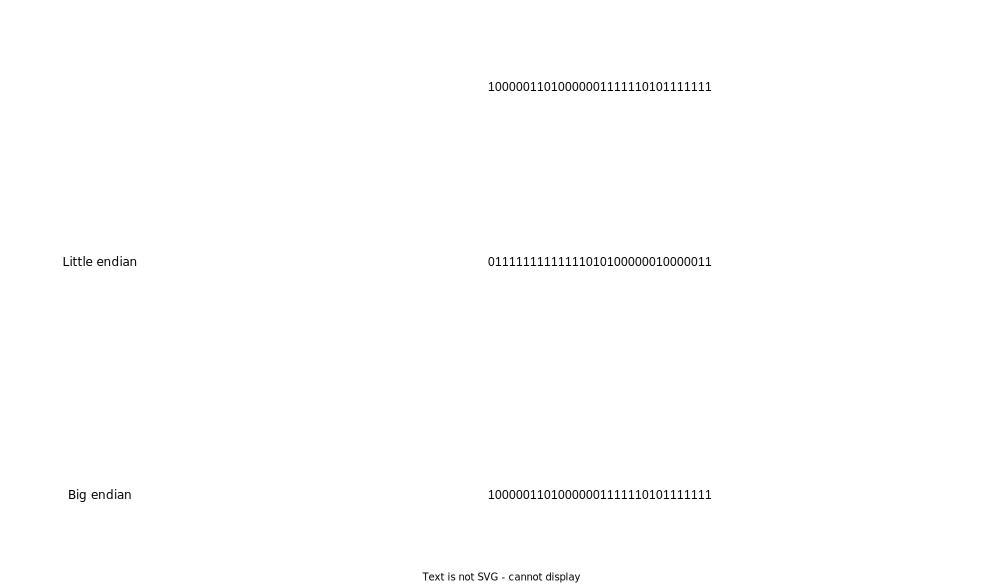
\includegraphics[width=\linewidth]{/Users/user/Documents/endianess.png}
  \caption{Endianess}
  \label{fig:endianess}
\end{figure}

    
  \subsection{Выравнивание}
    \begin{itemize}
      \item Числа быстрее считываются процессором, если они лежат по адресам, кратным их размерам
      \item Например: \cmint{sizeof(int)} = 4 $\Rightarrow$ выравнивание по границе 4 байт
      \item \cmint{char} -- 1 байт
      \item \cmint{short} -- 2 байта
      \item \cmint{int} -- 4 байта
      \item \cmint{long long} -- 4 байта
    \end{itemize}
    
    Работа с выровненными данными происходит быстрее.\\
    Есть архитектуры, которые в принципе не позволяют читать по невыровненным адресам, например, arm. В процессорах Intel можно сделать так же.
    
  \subsubsection{Выравнивание структур}
    \begin{itemize}
      \item Члены структур располагаются рядом
      \item Но если им не хватает выравнивания, компилятор ``добивает'' структуру pad'ами
      \item Выравнивание структуры -- максимальное выравнивание среди всех выравниваний её членов
    \end{itemize}
    
  \subsection{Знаковые числа}
  \subsubsection{One's complemnt}
    \begin{itemize}
      \item $-A = BitwiseNot(A)$
      \item Диапазон: $[-2^{N - 1} + 1, 2^N - 1]$
    \end{itemize}
    Преимущество такого представления: естественным образом реализуется сложение чисел. Однако есть проблема.
    \begin{itemize}
      \item $-1 = 1110$
      \item $+1 = 0001$
      \item $1110 + 0001 = 1111 = -0$
    \end{itemize}
    Получается 2 представления нуля. Это порождает еще проблемы:
    \begin{itemize}
      \item $-1 = 1110$
      \item $+2 = 0010$
      \item $1110 + 0010 = \textcolor{red}{1}0000 = 0$
      \item Упс...
    \end{itemize}
  
  \subsubsection*{One's complement: end-around-carry}
    \begin{itemize}
      \item Бит переноса отправляется назад, чтобы всё исправить
      \item $1110 + 0010 = \textcolor{red}{1}0000 = 0 + \textcolor{red}{1} = 1$
    \end{itemize}
  
  \subsubsection*{One's complement: недостатки}
    \begin{itemize}
      \item Два представления для $0$: $0000 = +0$ и $1111 = -0$
      \item End-around-carry
      \item Зато сложение и вычитания одинаковое для знаковых и беззнаковых чисел (почти)!
    \end{itemize}
  
  \subsubsection{Two's complement}
    \begin{itemize}
      \item Определение отрицательных чисел: $A + (-A) = 0$
      \item Давайте каждому положительному число сопоставим отрицательное
      \item $-A = BitwiseNot(A) + 1$
      \item Одно представление нуля: $-0 = BitwiseNot(A) + 1 = 1111 + 1 = 0000 = +0$
      \item Диапазон чуть больше, чем у one's complement: $[-2^N, 2^N - 1]$
      \item Используется в современных процессорах
    \end{itemize}
    
    Теперь мы можем складывать знаковые и беззнаковые числа абсолютно одинаково.
  
  \subsubsection*{Two's complement: недостатки}
    \begin{itemize}
      \item Операции сравнения теперь сложные
      \item Умножение требует sign extension: $0010 = 00000010, 1000 = 11111000$
      \item ``Перекос'' диапазона представимых чисел
      \item \cmint{abs(INT_MIN)} = ???
    \end{itemize}
  
  \subsection{Действительные числа}
  \subsubsection{Числа с фиксированной точкой}
    \begin{itemize}
      \item $N$ бит на целую часть, $M$ бит на дробную
      \item Всегда одинаковая точность
      \item Операции легко реализуются
    \end{itemize}
  
  \subsubsection{Числа с плавающей точкой}
  Раньше процессоры имели отдельную плату для операций с числами с плавающей точкой.
    \begin{itemize}
      \item IEEE 754
      \item Стандарт 1985 года
    \end{itemize}
  
    Числа с плавающей точкой представлены 3 частями:
    \begin{itemize}
      \item Представление: $(-1)^S \times M \times 2^E$
      \item $S$ -- бит знака, $M$ -- мантисса, $E$ - экспонента
      \item \cmint{float} (single): $|S| = 1$, $|M| = 23$, $|E| = 8$
      \item \cmint{double}: $|S| = 1$, $|M| = 52$, $|E| = 11$
    \end{itemize}
  
  \subsubsection*{Нормализованные значения}
    \begin{itemize}
      \item $|E| \neq 0$ и $E \neq 2^{|E|} - 1$
      \item Экспонента хранится со смещением: $E_{real} = E - 2^{|E| - 1}$
      \item Мантисса имеет ``виртуальную 1'': $M_{real} = 1.mmmmmmm$
    \end{itemize}
    
  \subsubsection*{Денормализованные значения}
    \begin{itemize}
      \item $E = 0$
      \item $E_{real} = 1 - 2^{|E|} = 1$
      \item Это самые близкие к нулю числа и сам ноль ($0.0$ и $+0.0$)
    \end{itemize}
  
  \subsubsection*{Специальные значения}
    \begin{itemize}
      \item $E = 2^{|E| - 1}$
      \item Если $M = 0$, то число представляет собой бесконечное значение
      \item Если $M \neq 0$, то число -- NaN
      \begin{itemize}
        \item[$\circ$] Используются при операциях с неопределенным значением: например, $sqrt(X)$, $\log(X)$, $X < 0$
      \end{itemize}
    \end{itemize}
    
  \subsubsection*{Проблемы IEEE 754}
    \begin{itemize}
      \item При вычислениях накапливается ошибка
      \item Сложение и умножение неассоциативно
      \item Умножение недистрибутивно
      \item NaN $\neq$ NaN (???)
      \item $0.0$ и $+0.0$
    \end{itemize}
  
  Более подробно о числах с плавающей точкой можно прочитать \href{http://steve.hollasch.net/cgindex/coding/ieeefloat.html}{здесь}.
  
  \subsubsection{Decimals}
    \begin{itemize}
      \item Представляются в виде двух чисел: $N$ -- знаменатель, $M$ -- числитель
      \item Все операции реализуются через приведение к общему знаменателю
      \item $N$ и $M$ обычно используют длинную арифметику, поэтому в теории точность ограничена только оперативной памятью
      \item Используются в финансах
    \end{itemize}
  
  \subsection{Кодировки}
    \begin{itemize}
      \item Умеем оперировать числами, но как перевести числа в текст?
      \item Кодировки -- ``карты'', сопоставляющие наборы байт каким-то образом в символы
    \end{itemize}
  
  \subsubsection{Немного терминологии}
    \begin{itemize}
      \item Character -- что-то, что мы хотим представить
      \item Character set -- какое-то множество символов
      \item Coded character set (CCS) -- отображение символов в уникальные номера
      \item Code point -- уникальный номер какого-то символа
    \end{itemize}
    
  \subsubsection{ASCII}
    \begin{itemize}
      \item American Standard Code for Information Interchange, 1963 год
      \item 7-ми битная кодировка, то есть кодирует 128 различных символов
      \item Control characters: с $0$ по $31$ включительно, непечатные символы, мета-информация для терминалов
    \end{itemize}
  
  \subsubsection{Unicode}
    \begin{itemize}
      \item Codespace: $0$ до 0x10FFFF ($\sim$1.1 млн. code points)
      \item Code point'ы обозначаются как U+<число>
      \item $\aleph$ = U+2135
      \item $r$ = U+0072
      \item Unicode -- не кодировка: он не определяет как набор байт трактовать как characters
    \end{itemize}
  
  \subsubsection{UTF-32}
    \begin{itemize}
      \item Использует всегда 32 бита (4 байта) для кодировки
      \item Используется во внутреннем представлении строк в некоторых языках программирования (например, Python)
      \item Позволяет обращаться к произвольному code point'у строки за $\mathcal{O}(1)$
      \item BOM определяет little vs. big-endian
    \end{itemize}
    Проблема: используется много места. Например, если мы пишем текст на английском, то под каждый символ будет выделено 4 байта, а можно было бы обойтись 1 (ASCII).
  
  \subsubsection{UTF-8}
    \begin{itemize}
      \item Unicode Transformation Format
      \item Определяет способ как будут преобразовываться code point'ы
      \item Переменная длина: от 1 байта (ASCII) до 4 байт
    \end{itemize}
    
    \begin{figure}[H]
    \centering
  \includegraphics[width=\linewidth]{/Users/user/Documents/utf8.png}
  \caption{UTF-8}
  \label{fig:utf8}
\end{figure}
  
  \subsubsection*{UTF-8 overlong encoding}
    \begin{itemize}
      \item $00100000$ = U+0020
      \item $11000000 \space 10100000$ = U+0020!
      \item overlong form или overlong encoding
      \item С точки зрения стандарта является некорректным представлением
    \end{itemize}